\section{Social and procedural aspects}

\subsection{Social dimensions}

\subsubsection{Overview}

Most often, negotiation takes place among people. Therefore, this process is a
social interaction and can be influenced by many social factors.
Social dimensions of negotiations are: Power, Influence, Status, Gender,
Ethics, Culture, etc.

\subsubsection{Power}

\begin{itemize}
    \item In the social sciences power is the ability to influence others
    \item It emerges from asymmetric control over valued resources in social
        relations (information, money, rhetorics, etc.)
    \item It is a potential force in a social relation, often not constant
        but dependent on the situation.
\end{itemize}

\paragraph{Types of power:}
\begin{itemize}
    \item Positional Power:
        \begin{itemize}
            \item Reward power: Based on the perception to have the ability to reward
            \item Coercive power: Based on the perception to have the ability to punish
            \item Legitimate power: Based on the perception to have a legitimate right
                to prescribe a behaviour (formal status, authority) 
        \end{itemize}
    \item Personal Power
        \begin{itemize}
            \item Referent power: Based on indentification and liking
            \item Expert power: Based on the perception to have special knowledge or
            expertness
        \end{itemize}
    \item Relational power: Based on relationships
\end{itemize}

\paragraph{Sources of Power:}
\begin{itemize}
    \item Positional power derives from the positions and roles you hold in
        your social system
    \item Personal power is derived from your unique set of personal attributs
        and skills
    \item Relational power is derived from your relationship with others.
        (This can provide emotional support, advice, information and other
        tangible resources)
\end{itemize}

\paragraph{Relevance for Negotiators}
\begin{itemize}
    \item Be aware of how much and what type of power you and the other party have
    \item The BATNA is one of the most important sources of power
        \begin{itemize}
            \item Know your BATNA and keep your options open
            \item Signal your BATNA /resistance point but do not reveal it
            \item Improve constantly your BATNA
            \item Asses the other sides BATNA
        \end{itemize}
    \item The contribtion to a negotiation is another source of power (bringing
        resources to the negotiation that are highly valued by the other side)
    \item Possible effects of power to those with more power:
        \begin{itemize}
            \item less accurate in assessing situations
            \item stronger illusion of control
            \item increased risk taking
        \end{itemize}
    \item Possible effects of power to those with less power:
        \begin{itemize}
            \item better in perceiving the behaviour of those with higher power
            \item fear of being constantly tested
            \item susceptible to the emotions of the other party
        \end{itemize}
\end{itemize}

\subsubsection{Influence and persuations}

\paragraph{Definition and Concept}

\begin{itemize}
    \item Social influence is the action of affecting the emotions, opinions,
        or behaviour of others
    \item One form of social influence, important for negotiation is persuasion
    \item Not only those with more power can be persuasive
    \item The two main streams of persuasion, build on:
        \item Rational and deliberate strategies based on information and
            arguments
        \item Credibility and likability. More of an automatic response to
            subtle cues.
\end{itemize}

\paragraph{Implications for Negotiators}
Information based persuation
\begin{itemize}
    \item \underline{Knowledge} of the negotiation subject is important
        \begin{itemize}
            \item You have to know the facts to be convincing
            \item Only a good understanding of the subject allows you
                to generate alternatives
        \end{itemize}
    \item Generate \underline{alternatives and options}:
        \begin{itemize}
            \item Consider alternatives
            \item Generate options (which sometimes are equally good for you)
        \end{itemize}
    \item $\rightarrow$ the one who formulates the alternatives may have an
        advantage
    \item Be aware of the \underline{power contrasts}. The perception of
        an offer can depend on:
        \begin{itemize}
            \item Previous offers
            \item Alternatives
        \end{itemize}
    \item $\rightarrow$ know what is good in absolute vs. relative terms
    \item Be aware of \underline{framing effects}. The perception of an offer
        can depend on how it is framed.
    \item $\rightarrow$ perception of gains and losses are different. It
        depends how a result is presented.
    \item Be aware of the \underline{anchoring effects}. In an experiment
        participants witnessed the spin of a manipulated roulette wheel
        (0 to 100). They were then asked whether they thought the percentage
        of the UN member countries coming from Africa is greater or smaller
        than the number on the wheel. Next, they were asked to make an
        estimation of the true percentage.
        \begin{itemize}
            \item Perticipants who saw the wheel stop on the number 10:
                guessed on average 25\%.
            \item Participants who saw the wheel stop on the number 65:
                guessed on average 45\%
        \end{itemize}
    \item $\rightarrow$ Tendency to give too much weight to the first offer.
        Try to re-anchor rapidly, as the agreement is often the midpoint between
        the first two offers.
    \item Be aware of the \underline{commitment and consistency principle}.
    \item $\rightarrow$ people often align with active commitments. Only commit
        to things you can stick to.
    \item Be aware of \underline{fairness heuristics}
        \begin{itemize}
            \item Offers labeled "fair" are more often accepted
            \item People tend to accept an offer made by themselves more often
                than an identical offer made by the other side
            \item There are different fairness principles:
                \begin{itemize}
                    \item Outcome is equally shared ("divide it down the middle")
                    \item Outcome is divided based on equity
                    \item Outcome is divided based on needs
                \end{itemize}
            \item Perception of fairness is subjective and depends on the
                circumstances (e.g. what others get)
        \end{itemize}
\end{itemize}

\paragraph{Emotion-based persuation}

\begin{itemize}
    \item Be aware of the \underline{principle of liking}
        \begin{itemize}
            \item We are more likely to comply with requests made by people
                that we like
            \item People like those who like them
            \item Liking is increased through similarity and praise
                \begin{itemize}
                    \item \underline{Similarity}: People were more willing
                        to buy an insurance policy from a salesperson who
                        was more akin to them in age, religion, politics, or
                        even cigarette-smoking habits.
                    \item \underline{Praise}: Experimental data show that
                        positive comments about another persons's traits,
                        attitute or performance reliably generates liking
                        in return and a willingness to comply with the
                        whishes of the person who is offering the praise.
                \end{itemize}
        \end{itemize}
    \item Be aware of the \underline{principle of social proof}
        \begin{itemize}
            \item $\rightarrow$ People follow th elead of similar others.
        \end{itemize}
    \item Be aware of \underline{appearance and judgment}
        \begin{itemize}
            \item Studies show that attrctive people tend to be perceived as
                more talented, kind, honest, intelligent, etc
        \end{itemize}
    \item Be aware of \underline{priming}
        \begin{itemize}
            \item Studies show that unconscious priming of cues in the envirnoment
                can influence the behaviour.
        \end{itemize}
    \item Be aware of \underline{time pressure}
        \begin{itemize}
            \item $\rightarrow$ often people abandon self-prescribed principles
                when hurried
        \end{itemize}
\end{itemize}

\paragraph{Persuation Frameworks}
Basic framework for individual level persuation:
Establish Credibility, Frame for common understanding, Provide evidence,
Connect emotionally.
Avice: Argue clearly and logically!

\subsubsection{Status}

\begin{itemize}
    \item Status is the relative position or rank given to people or groups
        by others
    \item Status influences social interactions, also through intervening,
        e.g. power or gender
    \item There are two types of statur characterisatics:
        \begin{itemize}
            \item Primary: rank, title (e.g. CEO), degree (e.g. PhD), etc
            \item Secondary: age, status in other groups, cultural background, etc
        \end{itemize}
\end{itemize}
Status exists in the eyes of others $>$ status perception can be changed.

How can you affect status perception in a negotiation?
\begin{itemize}
    \item Choose the right reference group
    \item Determine the reference group of your counterpart
    \item Use concerns about status strategically
    \item Seek out objective standards
\end{itemize}

\subsubsection{Gender}

\paragraph{Definition and Concept}

\begin{itemize}
    \item Between 1992 and 2019, women constituted, on average, 13\% of negotiators,
        6\% of mediators, and 6\% of signatories of major peace processes
        worldwide.
    \item Worldwide, women's representation in national parliament stands
        at $25\%$ in 2020.
    \item Among the G20 countries, the share of women in middle and senior
        management positions stands at 30\% in 2020.
    \item Gender: refers to the social attribute and opportunities associated
        with being male and female (UN Woman definition)
    \item Gender can have a strong influence on social interaction, status
        perception, and influencing processes
    \item What does research tell us on the role of gender in negotiations?
\end{itemize}

\paragraph{Research findings}

How well do different genders do at the bargaining table relative to one
another?
\begin{itemize}
    \item Women tend to set lower opening offers than men of similar
        experience, education and bargaining position
    \item Men tend to outperform in negotiation situations characterized
        by structural ambiguity
    \item Women are less likely to initiate negotiations than men e.g. for
        salary negotiations
\end{itemize}
How are men and women treated by their conterparties in negotiations?
\begin{itemize}
    \item Women encounter social and economic backlash when they behave
        assertive in negotiations
    \item Women who "ask" are viewed more negatively then men who ask (and
        more penalized by evaluatory)
    \item Self-advocating female negotiators suffer negative social judgment
\end{itemize}
Gender stereotypes are pervasice in our society but they do not represent reality:
\begin{itemize}
    \item \underline{Women}: gentle, not aggressive, submissive, talkative
        sensitive, emotional, verbal
    \item \underline{Men}: tough, aggressive dominant, not talkative, less
        sensitive, logical, analytical
\end{itemize}
They do not tell anything useful about the real world.
\begin{itemize}
    \item \underline{Effective negotiators} are characterized as: assertive, rational,
        decisive, constructive
    \item \underline{Ineffective negotiators} are regarded as: weak, emotional,
        irrational, too conciliatory
    \item Many of the traits that characterize effective negotiators are
        perceived to be masculine in nature, and many of the traits of
        ineffective negotiators are perceived to be feminin
    \item \underline{Stereotype threat}: a negative threat, whether or not
        endorsed by the holder, influences judgements and behaviour
    \item When stereotypes are explicitly activated, people exhibit
        \underline{stereotype reactance}
\end{itemize}

\paragraph{Implications for Negotiators}
Strategies to counteract the situation:
\begin{itemize}
    \item Regenerate stereotypes
        \begin{itemize}
            \item Members of traditionally stereotyped groups can redefine their
                own beliefs about their group.
            \item Stereotypes can be desmantled by openly addressing them
            \item Studies show that such practices can close the gap in
                negotiations
        \end{itemize}
    \item Redefine agency
        \begin{itemize}
            \item Members of traditionally stereotyped groups can assume
                a representation role in negotiations (for an organization,
                another person, a cause)
            \item Studies show that female negotiator's performance enhances
                when negotiating for someone else as opposed to only
                themselves
        \end{itemize}
    \item Prepare well
        \begin{itemize}
            \item Increase the degree of certainty in parties' understanding
                of the economic structurs in the negotiation (e.g. benchmark
                values)
            \item Studies show that gender differences in outcomes tend
                to be smaller when negotiators receive information about
                the bargaining range in negotiation simulations
        \end{itemize}
\end{itemize}
In professional negotiations, there should be no gender relevance.

\subsubsection{Ethics}

\paragraph{Definition and Concept}

\begin{itemize}
    \item Ethics are manifestations of cultural, contextual, and interpersonal
        norms that make certain strategies and behaviours unacceptable
    \item Negotiations can create incentives for people to violate ethical
        standards and negotiators must sometimes deal with an ambiguity of what
        is ethical
\end{itemize}

\paragraph{Lying}

\begin{itemize}
    \item Lying is regarded to be unethical (and in some cases illegal)
        \begin{itemize}
            \item Knowingly misrepresentation of a material fact is unethical
                and can be illegal
            \item Negotiations must happen in good faith but it is generally
                assumed that people are self-interested
            \item Misrepresentation of own interests is not lying about
                material facts and it is not illegal to exaggerate the own
                position
        \end{itemize}
    \item Omission vs. Commission
        \begin{itemize}
            \item Omission (Auslassung) = withholding relevant (or irrelevant)
                information $\rightarrow$ can be OK or is even a must, "Good
                negotiators need not disclose everything"
            \item Commision (Falschaussage) = active lying $\rightarrow$ not
                acceptable, "Good negotiators need not lie."
        \end{itemize}
\end{itemize}

Under what conditions do people engage in Deception?

\begin{itemize}
    \item Influencing factors that may lead people to engage in deception:
        \begin{itemize}
            \item Prospect of economic gain
            \item Uncertainty
            \item Anonymity of victims
        \end{itemize}
    \item Groups have a higher tendency to lie compared to individuals in the
        same bargaining situation.
\end{itemize}

\paragraph{Other questionable negotiation strategies}

\begin{itemize}
    \item Traditional competitive bargaining
        \begin{itemize}
            \item e.g. making very high or low opening offers (generally not
            regarded as unethical)
        \end{itemize}
    \item Manipulation of an opponent's network
        \begin{itemize}
            \item Trying to weaken an opponent by influencing his or her
                associate or constituency
        \end{itemize}
    \item Cancel a negotiated agreement
        \begin{itemize}
            \item Is it unethical to retract from an agreement after an informal
                closing has occured but while it is still legal (e.g. just
                before signing)
        \end{itemize}
    \item Retracting an offer
        \begin{itemize}
            \item Is it unethical to retract an offer made during a negotiation?
                Legal, but bargaining in bad faith
        \end{itemize}
    \item Small additions
        \begin{itemize}
            \item Strategy of continually asking for "just one more thing"
                after the deal has been closed.
        \end{itemize}
\end{itemize}

\subsubsection{Culture}

\paragraph{Definition and Concept}

\begin{itemize}
    \item Culture is shared patterns of values and norms learned through a
        process of socialization
    \item Culture is a unique characteristic of a social group (which does not
        have to be the nation state)
    \item Culture influences our mental models of how things work
    \item But differences within cultures can be significant
\end{itemize}

\begin{figure}[h]
    \centering
    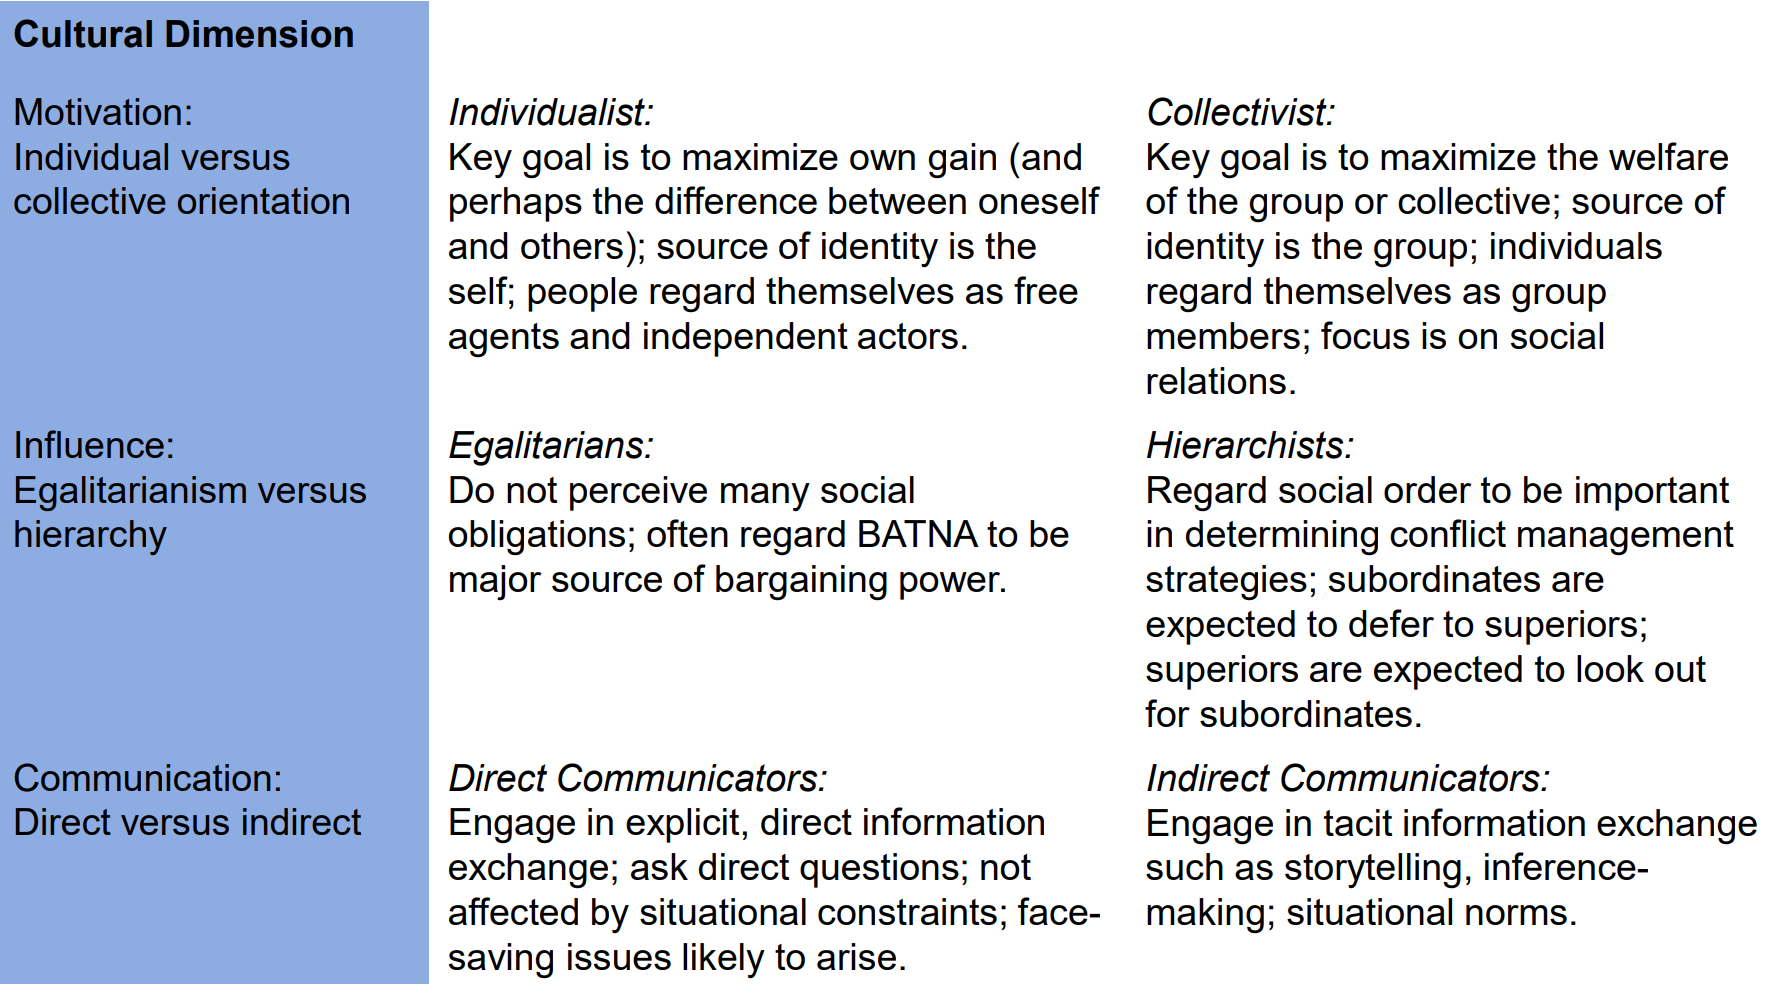
\includegraphics[width=0.8\textwidth]{Pictures/Possible_cultural_dimensions_of_interest.png}
\end{figure}

\paragraph{Implications for Negotiators}

\begin{itemize}
    \item Know where you are in the negotiation process:
        \begin{itemize}
            \item Building a relationship
            \item Exchanging information
            \item Trying to persuade each other
            \item Making concession and reaching an agreement
        \end{itemize}
    \item Concentrate on the commonality rather than on the differences:
        \begin{itemize}
            \item politeness
            \item respect
            \item and a sense of humor
            \item The above three points are appropriate in all culturse!
        \end{itemize}
    \item Some questions to ask yourself:
        \begin{itemize}
            \item How does the other side perceive my culture?
            \item How does the other side perceive power?
            \item How does the other side perceive time?
            \item Does the other side communicate directly or implicitly?
            \item How do you show respect?
        \end{itemize}
    \item Some remarks for overcoming cultural differences:
        \begin{itemize}
            \item Learn the other side's culture (part of the preparation)
            \item Don't stereotype (there is still variance)
            \item Be aware of your own culture and how others may perceive it
            \item Find ways to bridge the cultural gap
        \end{itemize}
\end{itemize}


\subsection{Procedural aspects}

Procedure can shape and influence the negotiations
\begin{itemize}
    \item Preparation
    \item Location
    \item Communication
    \item etc.
\end{itemize}

\paragraph{Steps of the negotiation process}

\begin{enumerate}
    \item Recognize/identify the problem
    \item Explore negotiation possibilities
    \item Get a mandate
    \item Negotiate within your mandate. If you have to change the mandate,
        you should be sure, that it is final.
    \item Initial the negotiation text, if practice (Up to here as a negotiator)
    \item Signing of the negotiation text
    \item Approval, if necessary
    \item Entry into force
    \item \textit{Open the champagne}
\end{enumerate}

\paragraph{Preparation of Negotiations}

\begin{itemize}
    \item Explore the situation well: Get the maximum of information on:
        \begin{itemize}
            \item Problem
            \item The other side's position
            \item Your possibilities
        \end{itemize}
    \item Mandate-drafting is decisive:
        \begin{itemize}
            \item Draft it yourself, if possible
            \item Mandate should be ambitious, but reasonable/realistic so that
                later adaptations do not become necessary.
        \end{itemize}
    \item For each round of negotiation prepare:
        \begin{itemize}
            \item 3 main questions:
                \begin{itemize}
                    \item What do you want to achieve?
                    \item How do you want to proceed?
                    \item Which follow-up?
                \end{itemize}
            \item Additional preparations:
                \begin{itemize}
                    \item Organization of your team (who speaks?)
                    \item Where?
                    \item Style of the negotiation?
                    \item Protocol
                    \item Communications and press information
                \end{itemize}
        \end{itemize}
\end{itemize}

\paragraph{Aspects regarding negotiation strategy: Question for avoiding
common mistakes in negotiation}

\begin{itemize}
    \item Are you pursuing a negotiated course of action only to justify an
        earlier decision?
    \item Are you assuming that what's good for you is necessarily bad for your
        opponent, and vice-versa?
    \item Are you being irrationally affected by an initial anchor price?
    \item Is there another frame that would put a different perspective on the
        negotiation?
    \item Are you being affected by readily available information, and ignoring
        other valid, but less accessible data?
    \item Have you fully thought about the decisions of your opponent?
    \item Are you placing too much confidence in your own fallible judgement?
\end{itemize}

\paragraph{Communication}

Verbal communication:
\begin{itemize}
    \item Use decent language
    \item Try to say it positively ("glass is half full")
\end{itemize}

\begin{table}[h]
    \begin{tabular}{c|c}
        Instead of this\dots & say this\dots \\ \hline
        Cririque & Comment \\
        Debate & Discuss \\
        Focus on differences & Search for common ground \\
        Fight & Discussion \\
        The opposition party & The other party \\
        No & Yes, but (e.g. "while I understand your position, I would like to
            emphasize...")
    \end{tabular}
\end{table}

Nonverbal communication

\begin{itemize}
    \item Appearance (cultivated, appropriate)
    \item Body language (gestures, body postures, facial expression)
    \item It is important to be aware of this communication especially in the
        other team. This can give you additional information ("face-to-face" in
        the same room is crucial for important negotiations (no tele-negotiations))
    \item Try to avoid judging according to simplified stereotypic ideas.
\end{itemize}

\paragraph{Location and physical environment}

\begin{itemize}
    \item Seating order always according to objective criteria:
        \begin{itemize}
            \item Alphabet
            \item Hierarchy
            \item Seniority
        \end{itemize}
\end{itemize}

\paragraph{Time}

\begin{itemize}
    \item Time can be source of power and leverage
    \item But also an obstacle
    \item Try to use deadlines in order to force the parties to be more constructive
        and to give up their resistance (Exp. Lausanne Iran - P5+1 Agreement 02.04.2015)
    \item But do not say the deadline will never be prolonged (In the sense of
        a "last chance")
\end{itemize}

\paragraph{Conclusion}

\begin{itemize}
    \item The procedure of a negotiation can be an important influencing factor
    \item It is important to manage it carefully
    \item Try to be:
        \begin{itemize}
            \item prepared
            \item goal oriented and objective
            \item intelectually skeptical and distrustful
            \item polite
        \end{itemize}
\end{itemize}
